\documentclass[12pt]{article}
\usepackage[spanish,activeacute]{babel}
\usepackage{graphicx}
\usepackage{wrapfig}
\usepackage[utf8]{inputenc}
\usepackage[margin=3cm]{geometry}
\usepackage{hyperref} 

\begin{document}


\begin{picture}(18,4)
\put(140,-220){
\includegraphics[width=5cm,height=5cm]{espol.png}}
\end{picture}

\begin{center}


\textbf{{\Huge Escuela Superior Politécnica del Litoral}\\[7cm]
{\LARGE Lenguajes de Programación}}\\[3.5cm]

{\LARGE \textbf{Manual de Usuario}}\\[1.5cm]
{\large Charlie Medina \\Joseph Gallardo\\ Kevin Zambrano}\\[2cm]
Ingeniería en Ciencias Computacionales\\[1cm]
Guayaquil - \today
\end{center}



\title{\bfseries\Huge Sudoku\\ Manual de usuario}

\date{}



\begin{minipage}{0.55\textwidth}
\begingroup
\let\center\flushleft
\let\endcenter\endflushleft
\maketitle

\endgroup
\end{minipage}
\begin{minipage}{0.1\textwidth}
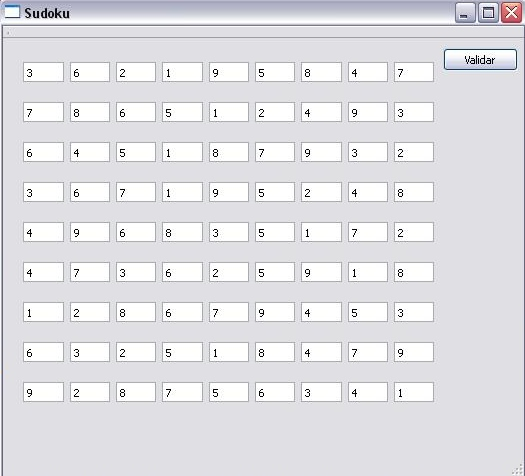
\includegraphics[height=6cm,width=8cm]{sudoku} 


\end{minipage}





\section{Introducción}

Sudoku es un pasatiempo que se publicó por primera vez a finales de la década de 1970 y se popularizó en Japón en 1986, dándose a conocer en el ámbito internacional en 2005 cuando numerosos periódicos empezaron a publicarlo en su sección de pasatiempos. El objetivo del sudoku es rellenar una cuadrícula de 9 x 9 celdas (81 casillas) dividida en subcuadrículas de 3 x 3 (también llamadas "cajas" o "regiones") con las cifras del 1 al 9 partiendo de algunos números ya dispuestos en algunas de las celdas, y lo característico del juego es llenar las casillas vacías con números que no se  repitan en una misma fila, columna o subcuadrícula. 
	

\section{Controles\\}

El juego no posee controles muy sofisticados, ya que solo se colocan dígitos del 1 al 9 en las casillas que se requieren llenar.
Por estar aún el juego en su proceso de desarrollo, no consta con los controles para llenar cada casilla.
Actualmente el juego solo posee un botón ‘validar’ el cual valida todas las casillas del tablero cumpliendo las restricciones de fila, columna y subcuadrícula.


\section{Interfaz}
La interfaz del juego; por estar aún en desarrollo, posee una interfaz muy casual, mostrando el tablero con sus  81 casillas teniendo algunas previamente llenas y otras vacías para ser completadas según la regla del juego.





\end{document}